\section{Experimental Results}

\begin{frame}
\frametitle{Experimental Results}
\framesubtitle{Implementation}

\begin{columns}
	\begin{column}{0.55\textwidth}
		\footnotesize
		\begin{itemize}
			\setlength\itemsep{0.1em}
			\item<1-> \textcolor{tudblue}{\textbf{Domain}}: Mobile Robot Navigation
			\vspace{10pt}
			\item<2-> Execution traces with odometric readings
			\item<2-> State space discretized by unsupervised machine learning ($k$-Means, GMM)
			\item<2-> Transition probabilities of MDPs computed by maximum likelihood
			\vspace{10pt}
			\item<3-> Performance assessed through simulations
			\item<3-> Tested on small and large environment
			\item<3-> \textbf{Software}: Python, ROS, \textit{Morse} simulator
		\end{itemize}
	\end{column}
	\begin{column}{0.5\textwidth}
		\centering
		\includegraphics<1->[width=\linewidth]{figures/implementation/render_2}
		\captionof*{figure}{\scriptsize\textit{\textcolor{tudBlack}{SCITOS-A5 mobile robot in a Morse simulation of the \texttt{uol\_bl} environment}}}
	\end{column}
\end{columns}

% How was our solution tested/evaluated?
% What experiments have been done?
% Which observations were made from the results?

\end{frame}

\begin{frame}
	\frametitle{Experimental Results}
	\framesubtitle{Demonstration [1/2]}
	\vspace{-15pt}
	\begin{center}
		\hspace{7pt}\includegraphics[width=0.65\textwidth]{figures/implementation/demo_clustering_v2.pdf}
	\end{center}
\end{frame}

\begin{frame}
	\frametitle{Experimental Results}
	\framesubtitle{Demonstration [2/2]}
	%\vspace{-15pt}
	\begin{center}
		\includegraphics[width=0.7\textwidth]{figures/implementation/tum_kitchen_render_trajectory_v8_high}
	\end{center}
\end{frame}

\begin{frame}
	\frametitle{Experimental Results}
	\framesubtitle{Base Framework - Small Environment - Dataset Size}
	\vspace{10pt}
	\begin{columns}
		\begin{column}{0.5\textwidth}
			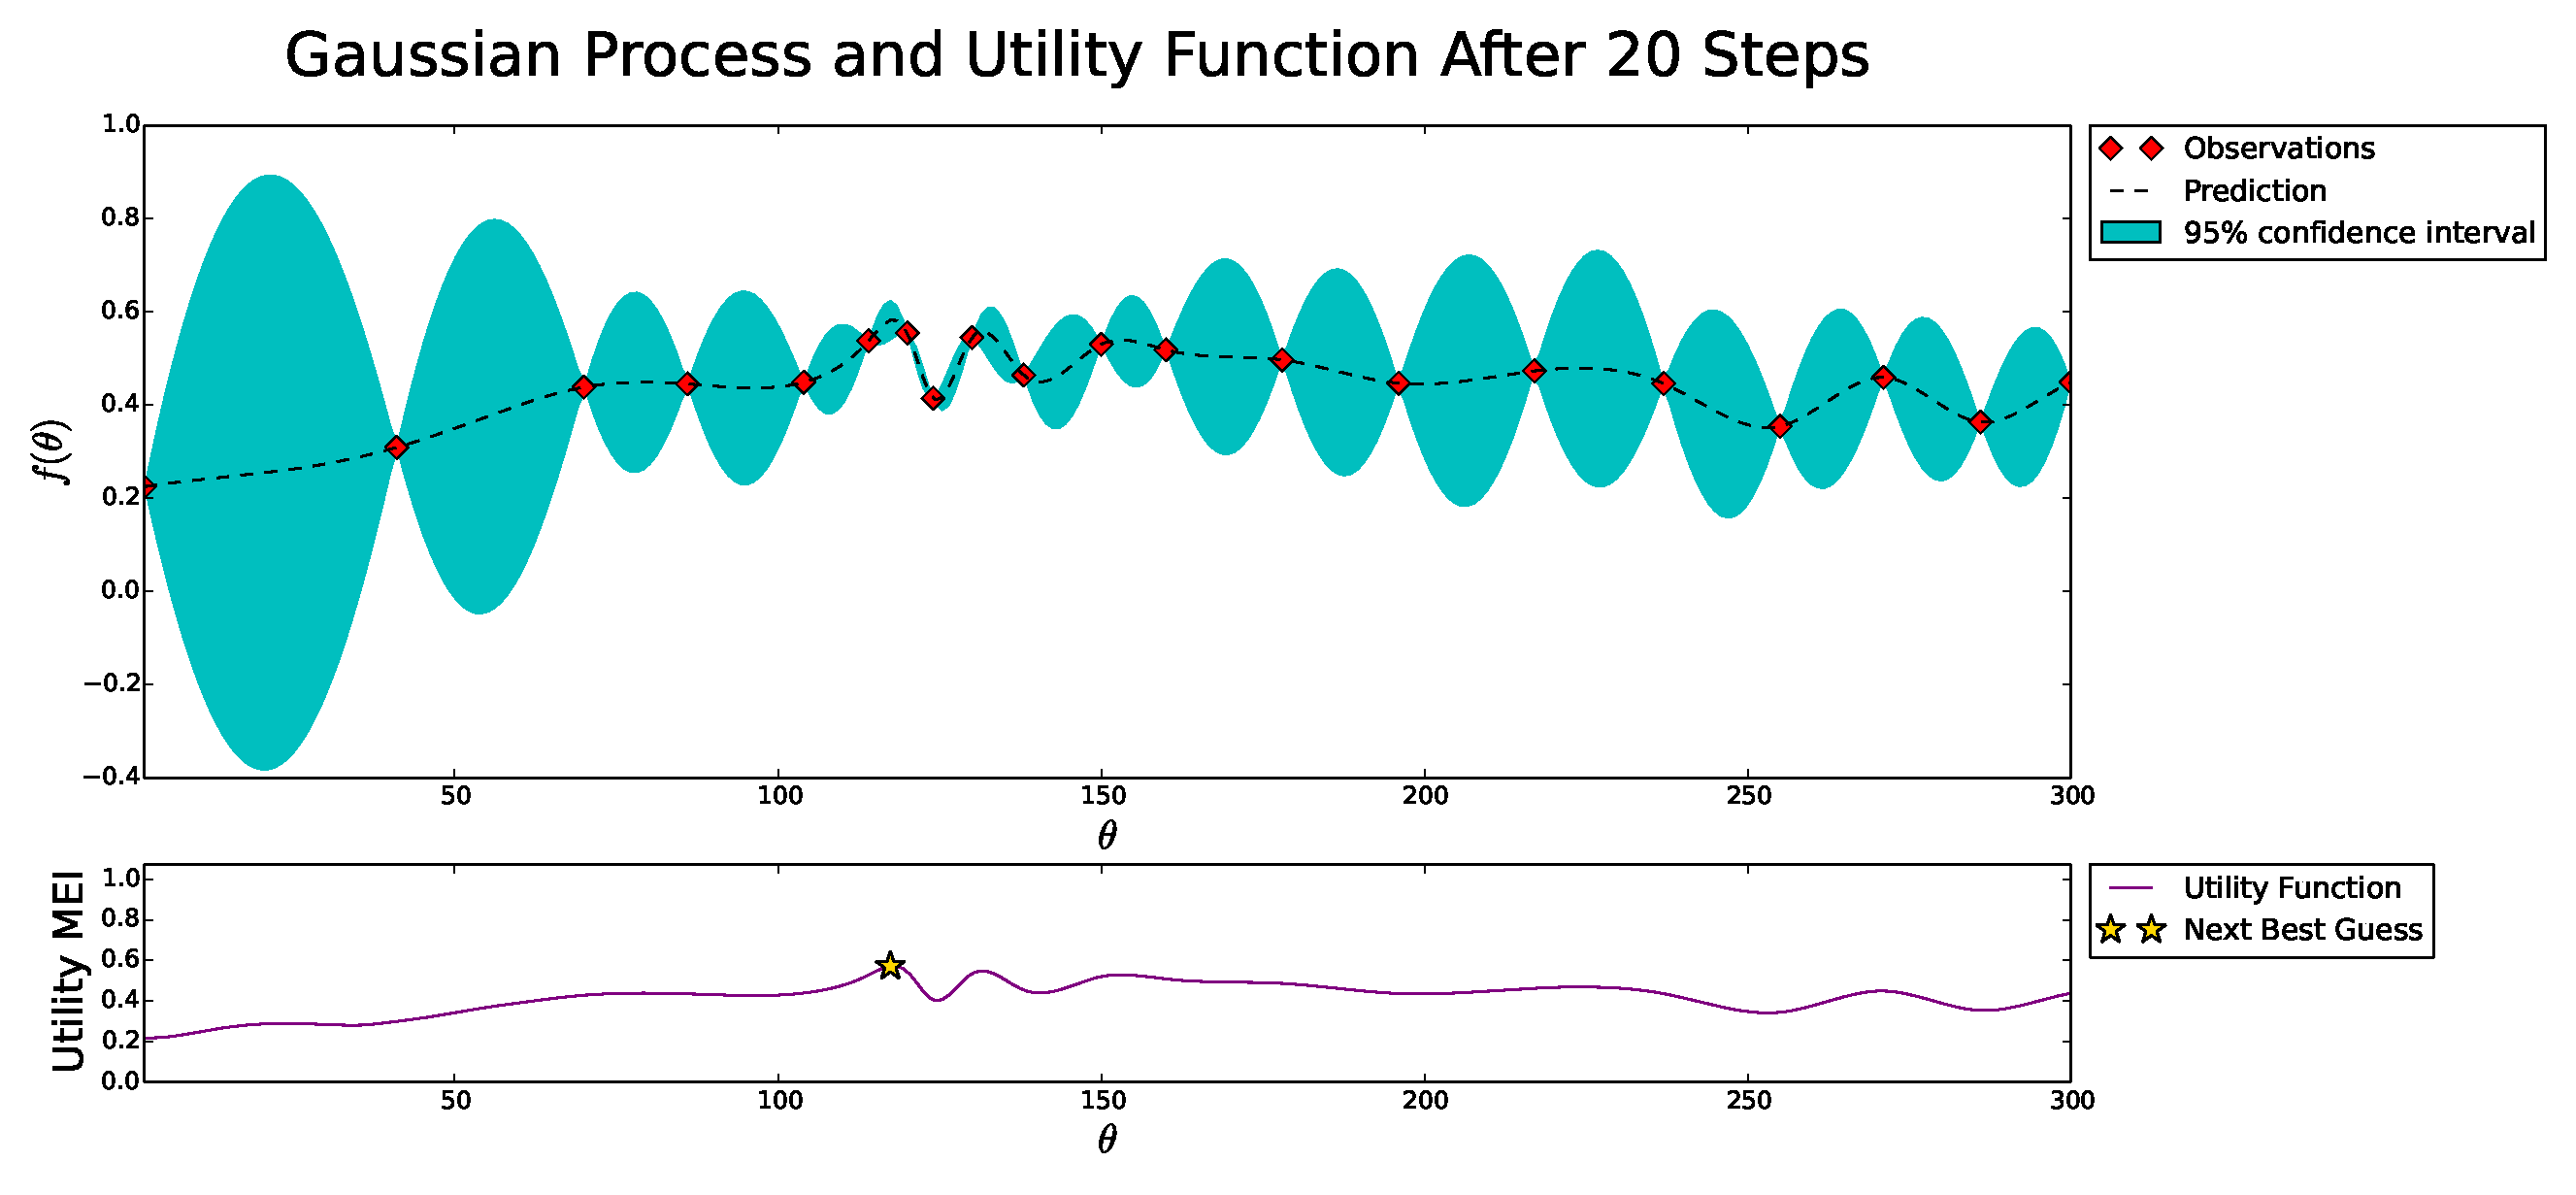
\includegraphics[width=\linewidth]{../../figures/plots/tum_base/plot_b_00__alg_kmeans_pct_100_acq_ei}
		\end{column}
		\begin{column}{0.5\textwidth}
			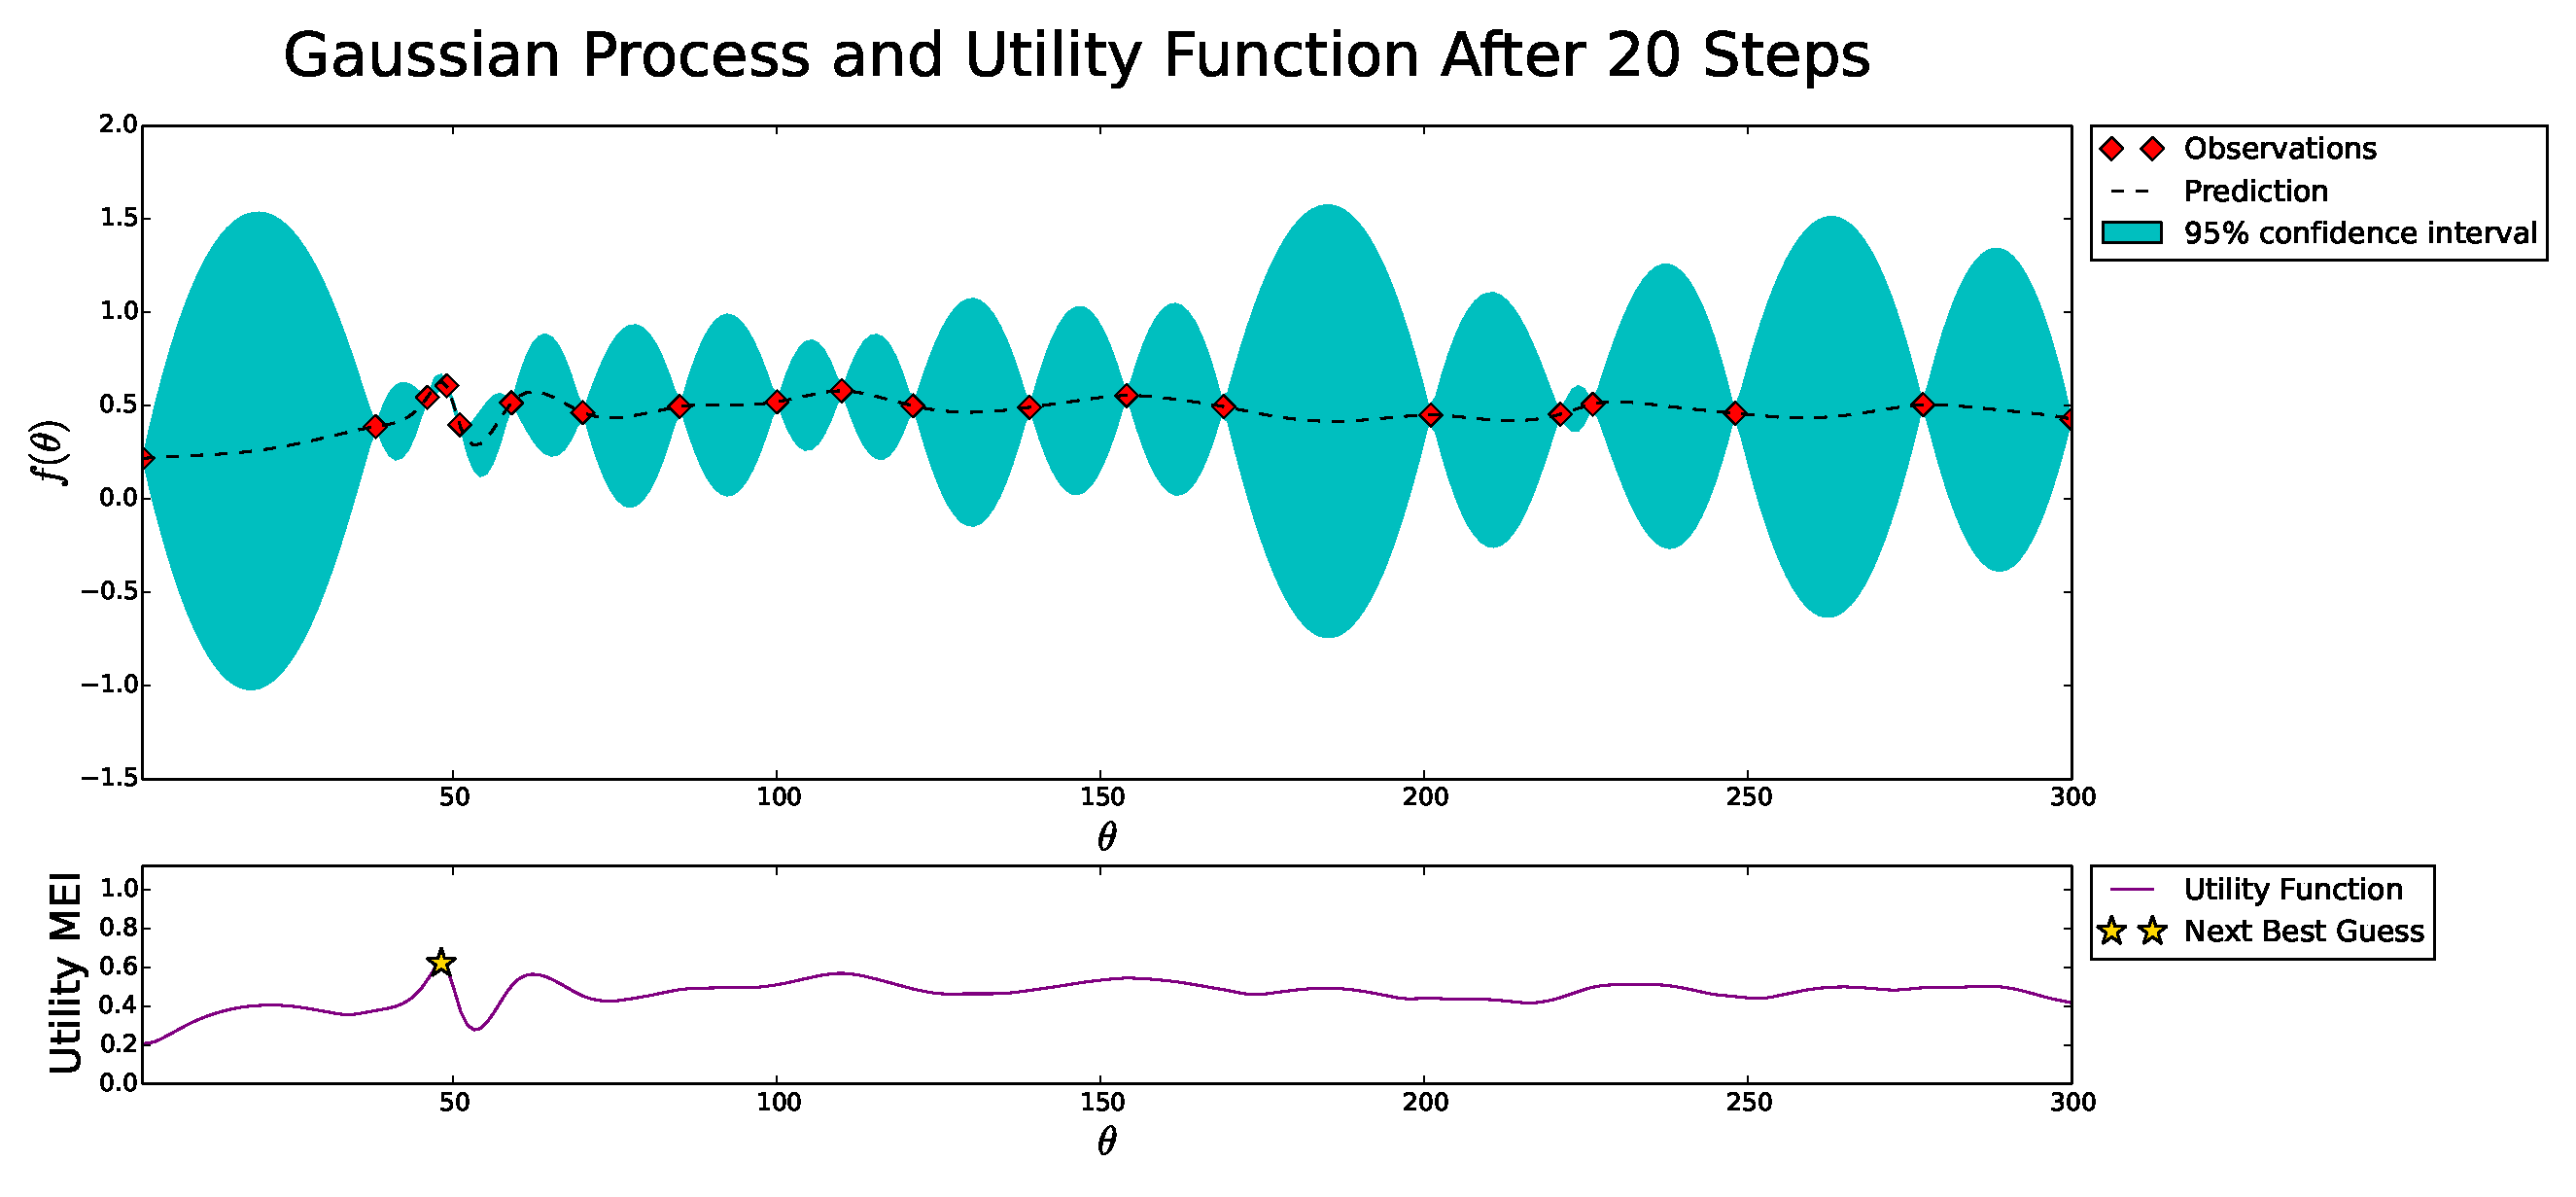
\includegraphics[width=\linewidth]{../../figures/plots/tum_base/plot_b_00__alg_kmeans_pct_50_acq_ei}
		\end{column}
	\end{columns}
	\begin{center}
		\footnotesize
		Resulting GP approximation with 100\% and 50\% of our dataset used\\
		($k$-Means, \texttt{tum\_kitchen} environment, EI acquisition, 20 iterations)
	\end{center}
\end{frame}

\begin{frame}
	\frametitle{Experimental Results}
	\framesubtitle{Base Framework - Small Environment - $\beta$ factor}
	\vspace{10pt}
	\begin{columns}
		\begin{column}{0.5\textwidth}
			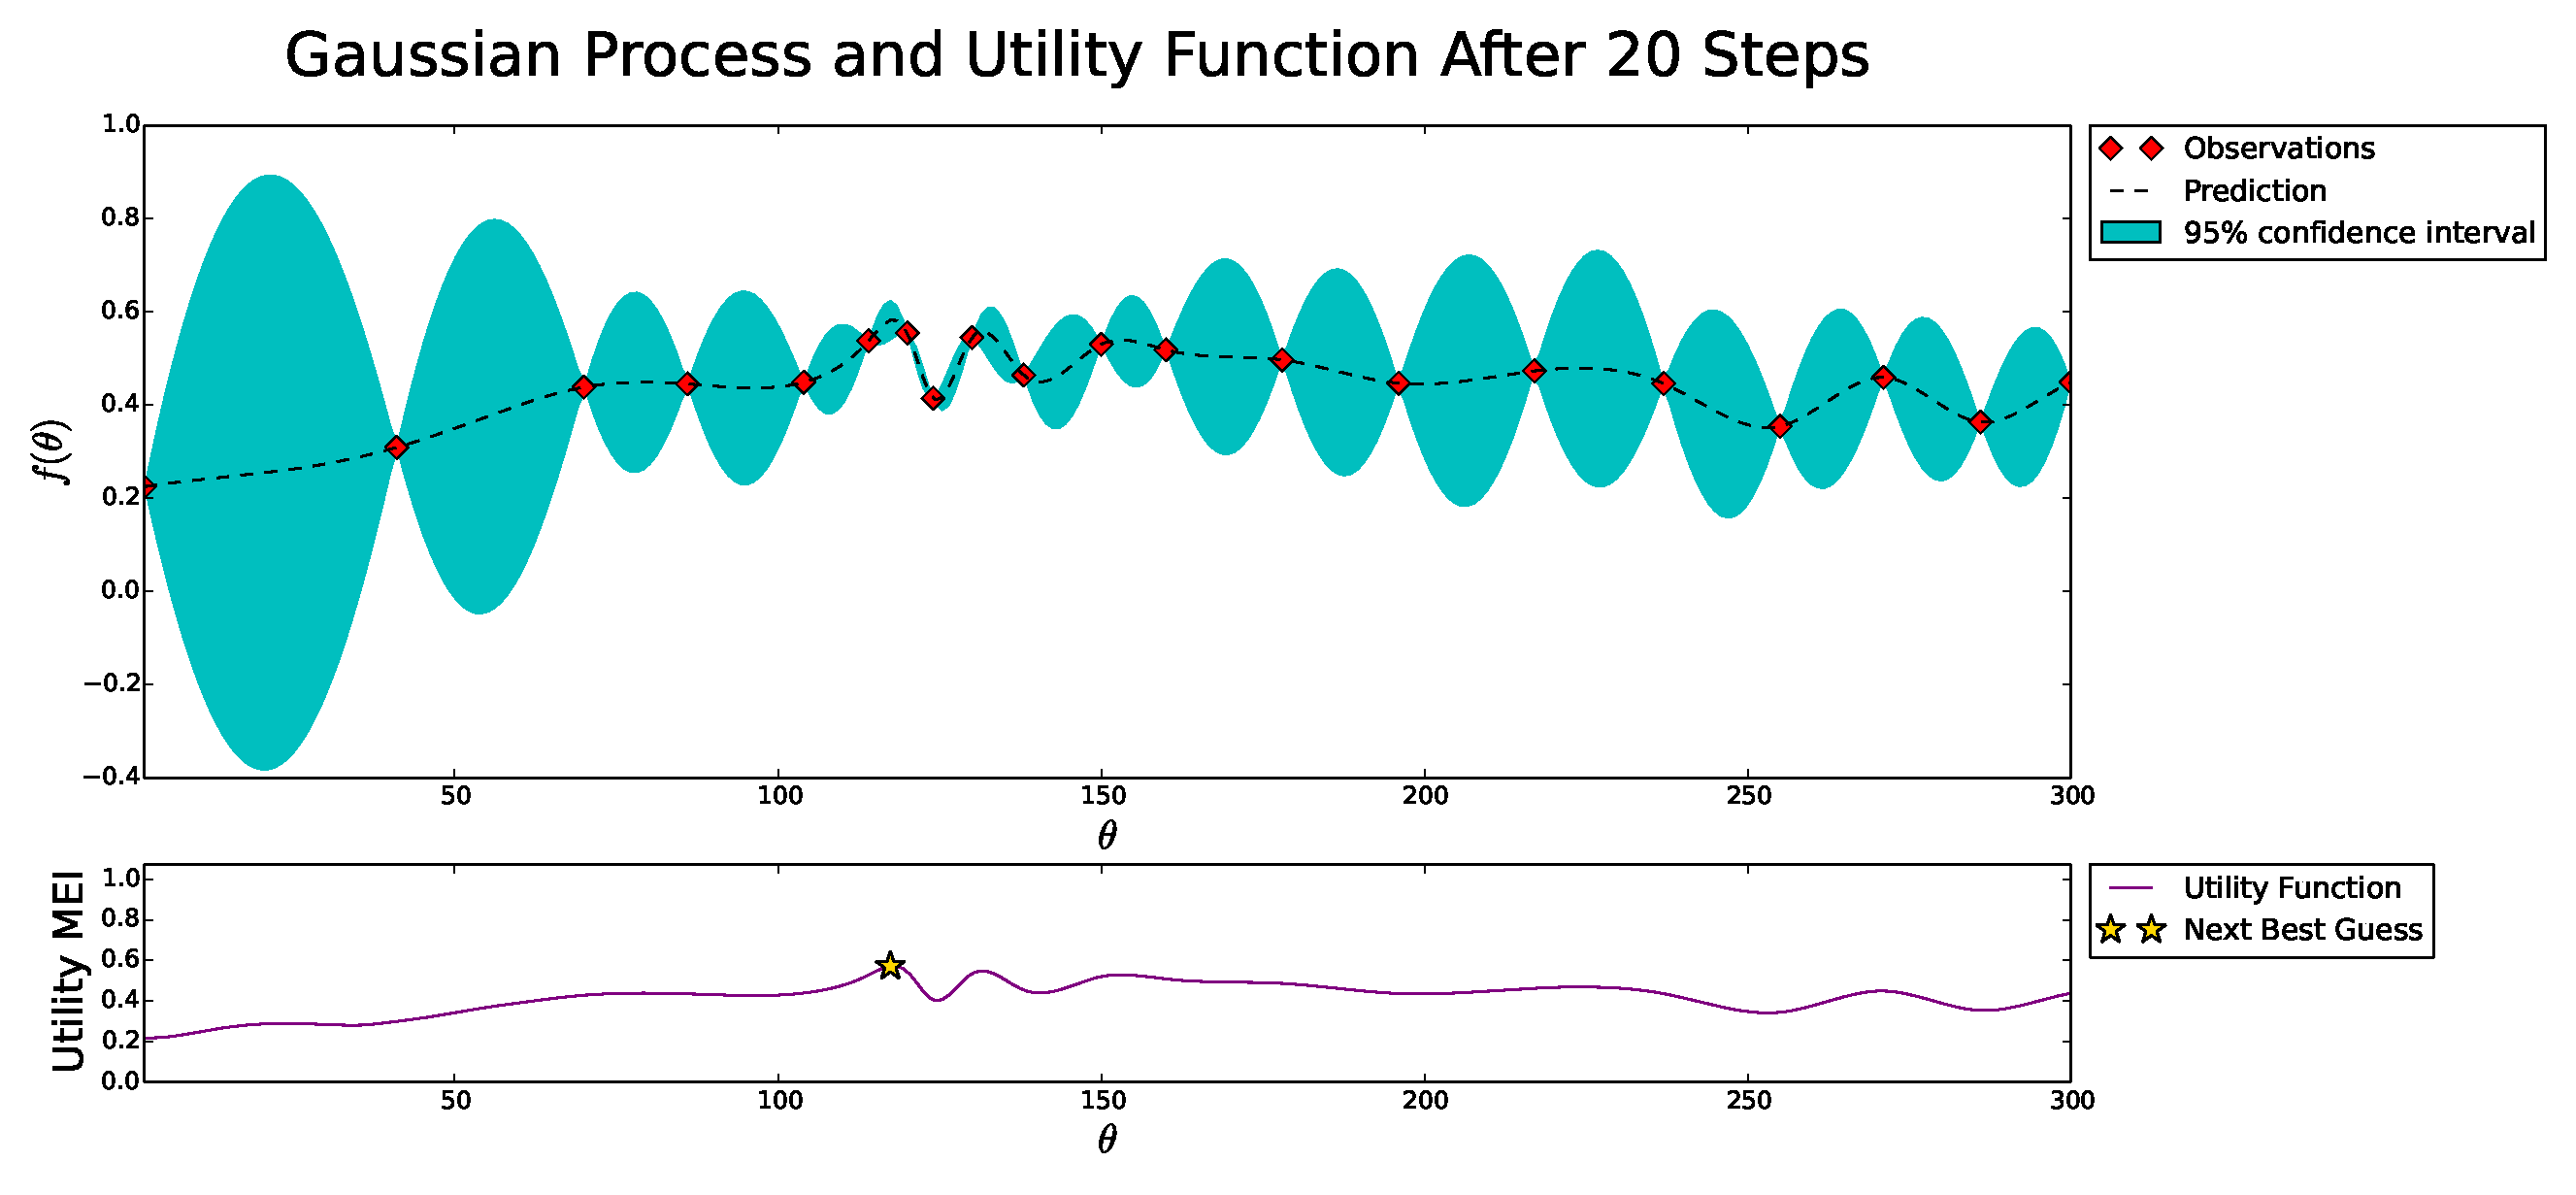
\includegraphics[width=\linewidth]{../../figures/plots/tum_base/plot_b_00__alg_kmeans_pct_100_acq_ei}
		\end{column}
		\begin{column}{0.5\textwidth}
			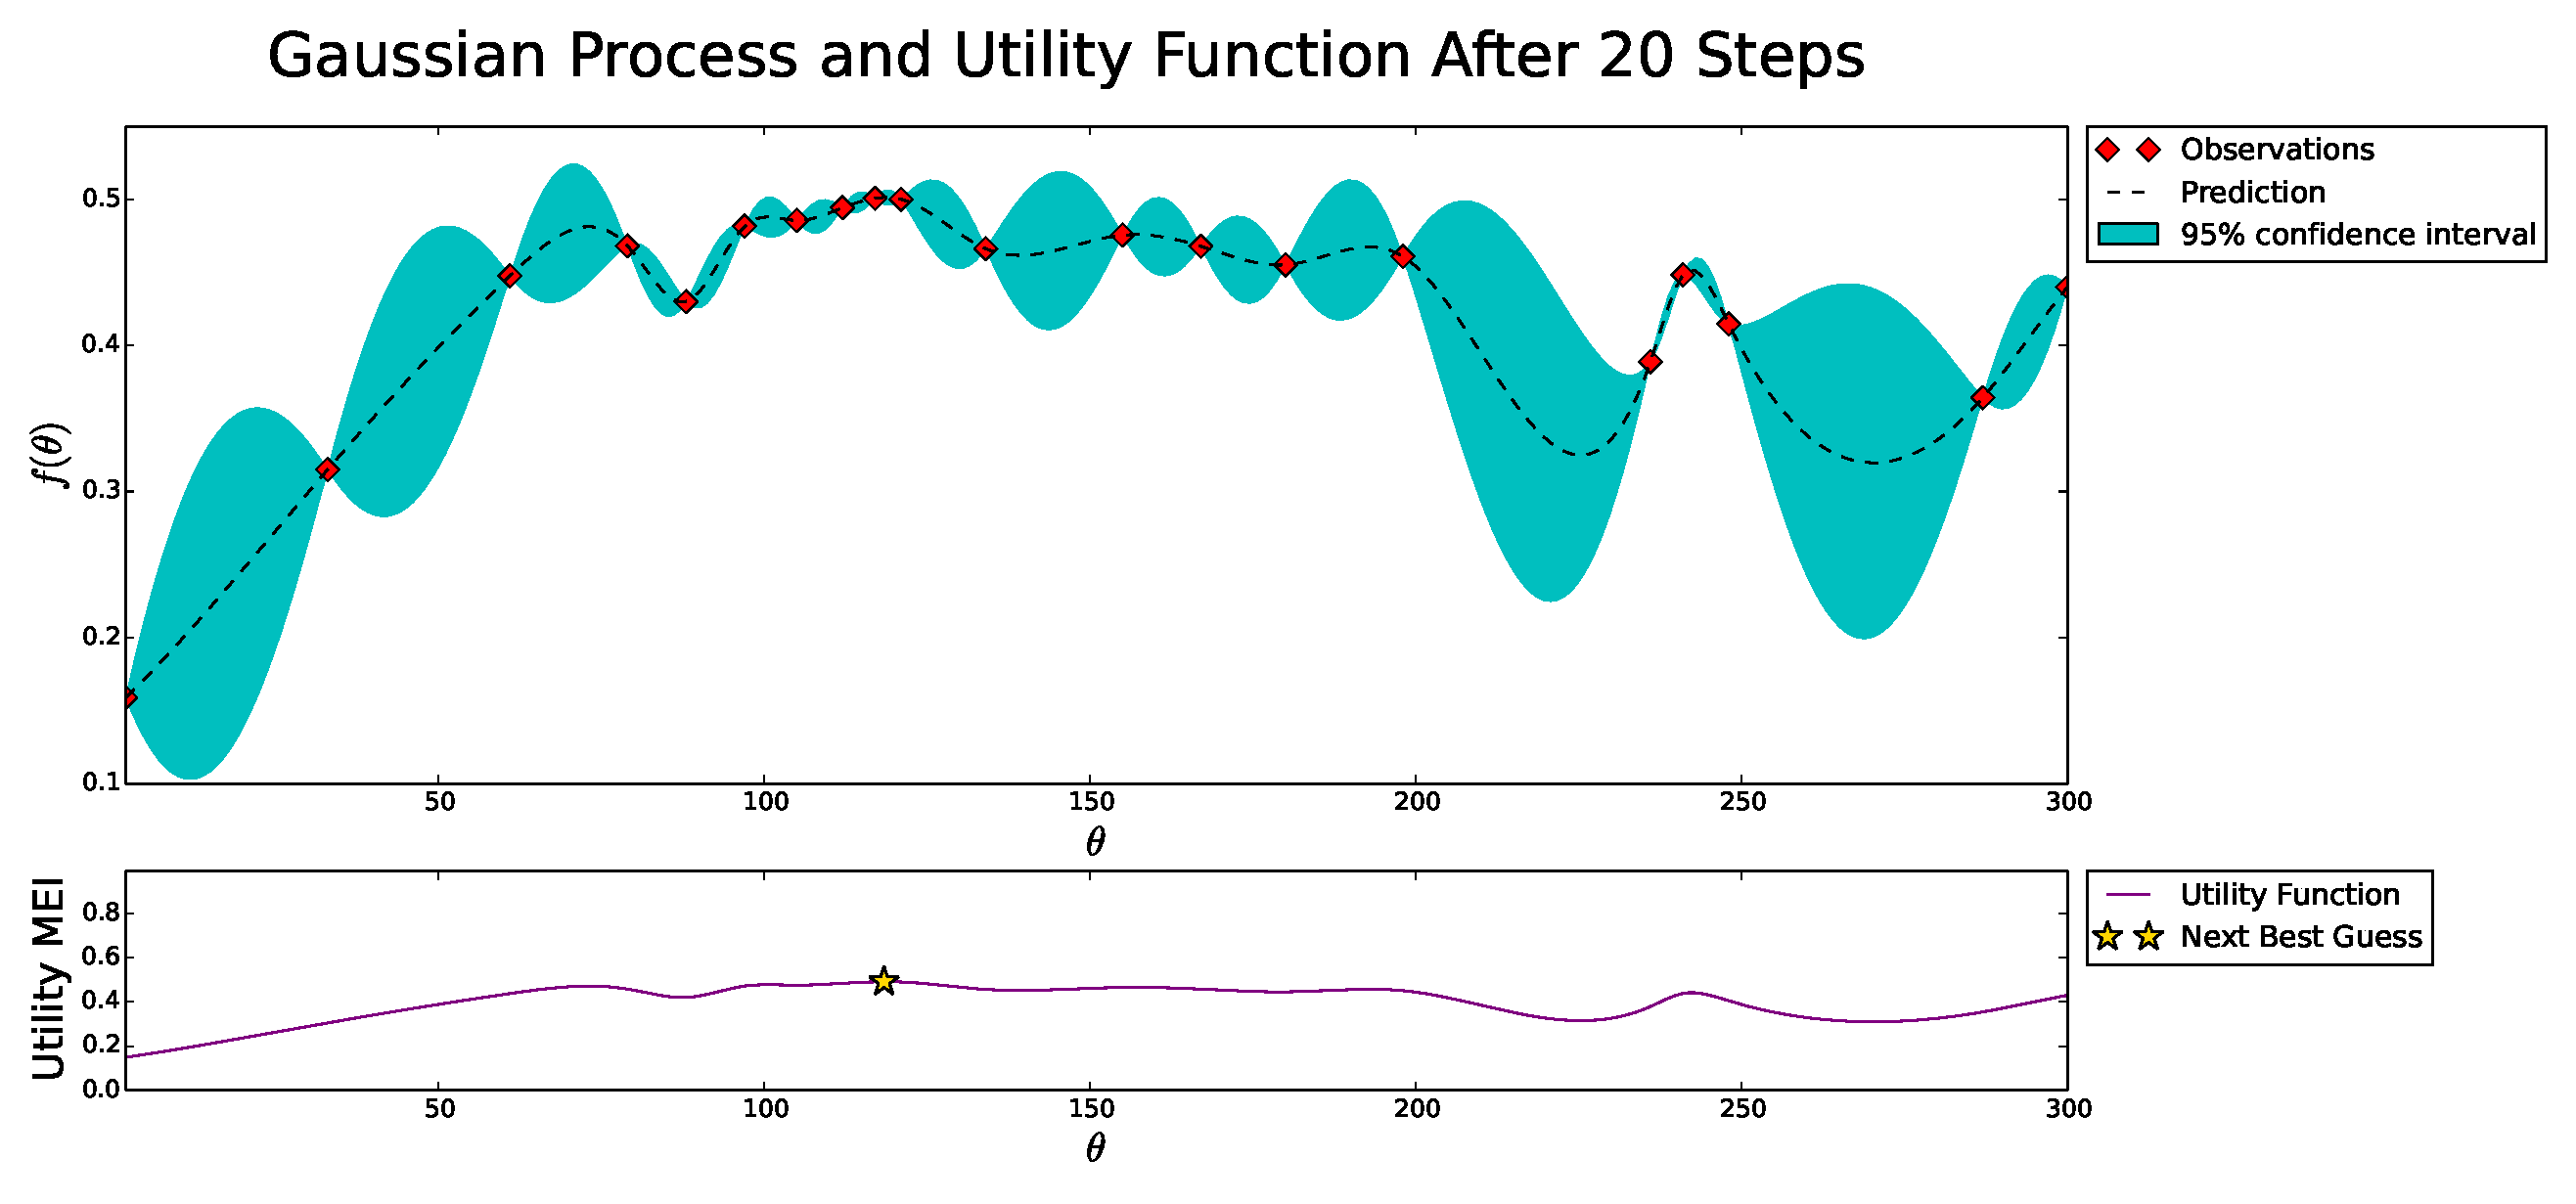
\includegraphics[width=\linewidth]{../../figures/plots/tum_base/plot_b_05__alg_kmeans_pct_100_acq_ei}
		\end{column}
	\end{columns}
	\begin{center}
		\footnotesize
		Resulting GP approximation with $\beta = 0.0$ and $\beta = 0.5$\\
		($k$-Means, \texttt{tum\_kitchen} environment, EI acquisition, 20 iterations, 100\% dataset used)
	\end{center}
\end{frame}

\begin{frame}
	\frametitle{Experimental Results}
	\framesubtitle{Base Framework - Large Environment}
	\vspace{10pt}
	\begin{columns}
		\begin{column}{0.5\textwidth}
			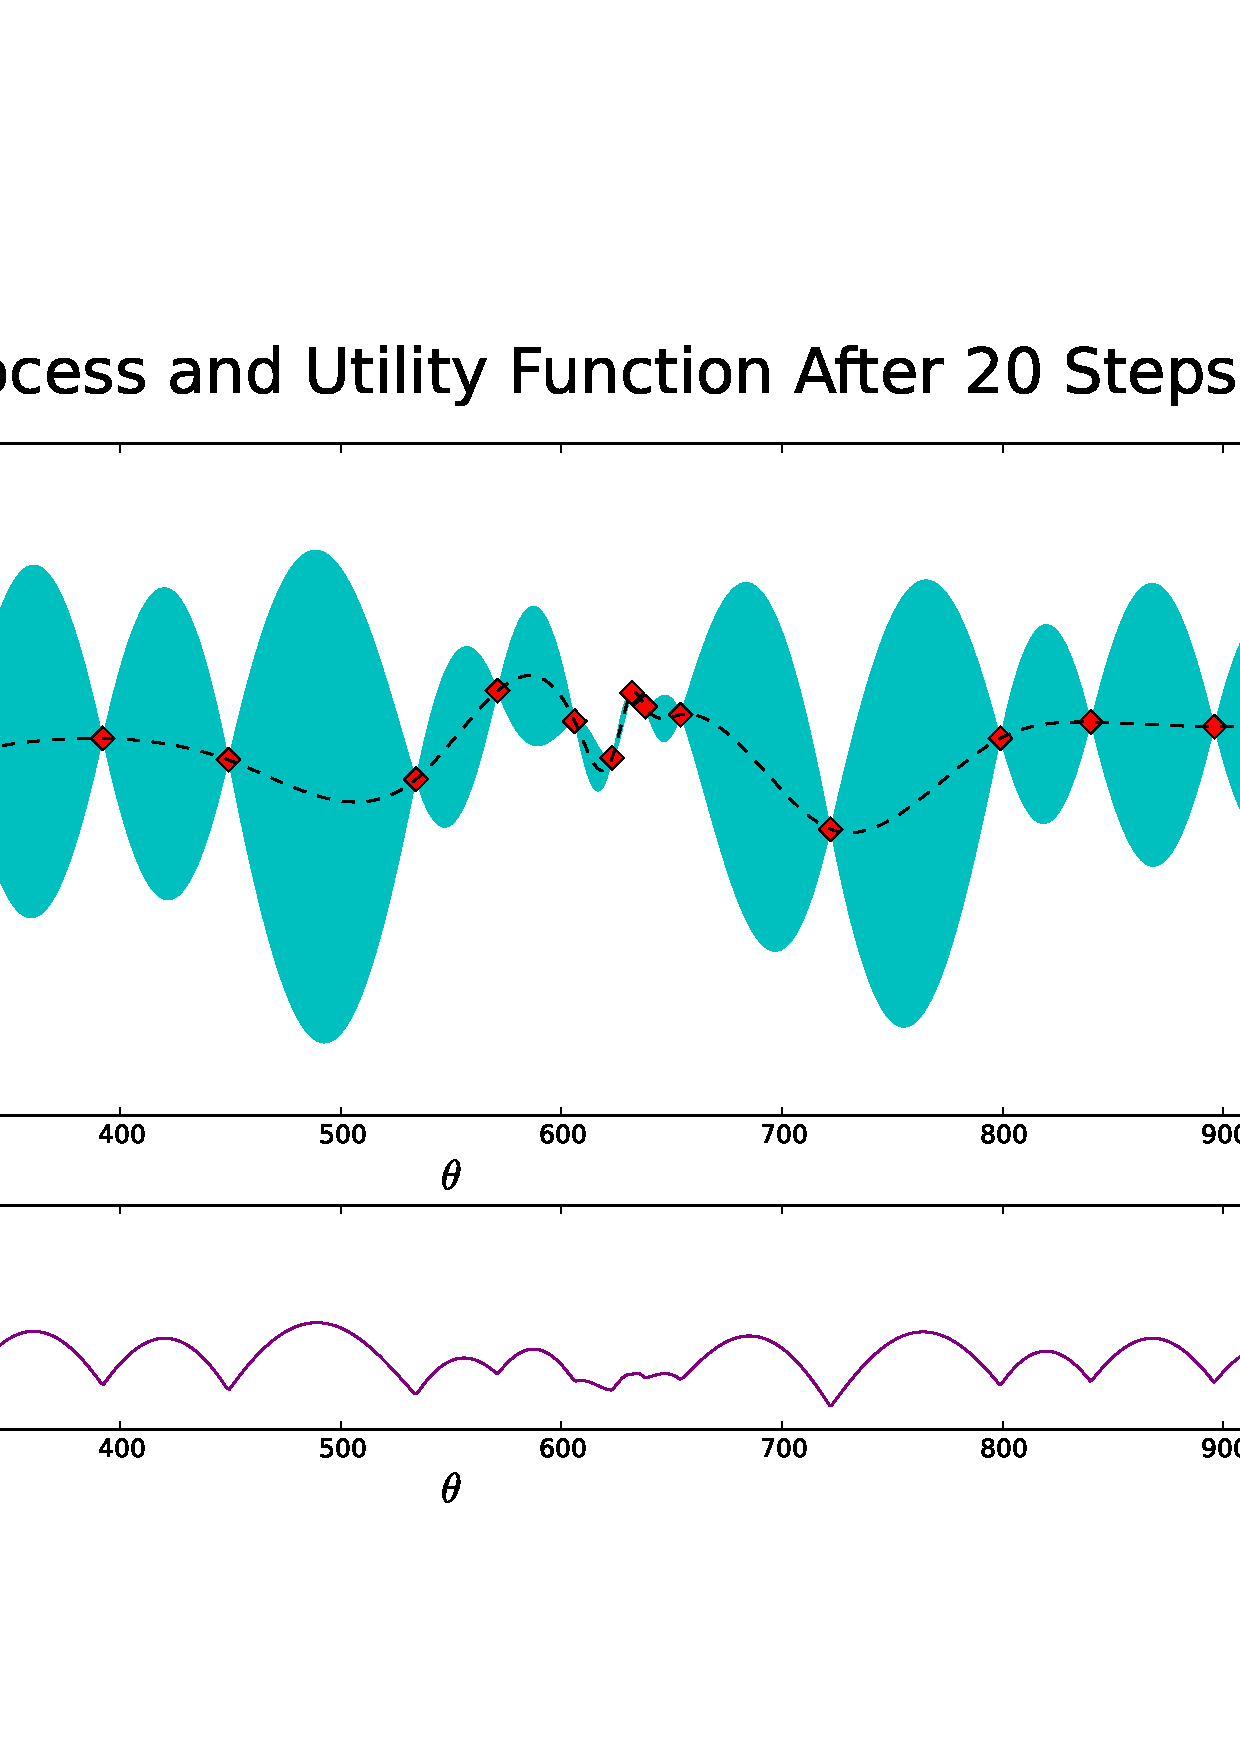
\includegraphics[width=\linewidth]{../../figures/plots/uol_base/plot_b_00__alg_kmeans_pct_100_acq_ucb.pdf}
		\end{column}
		\begin{column}{0.5\textwidth}
			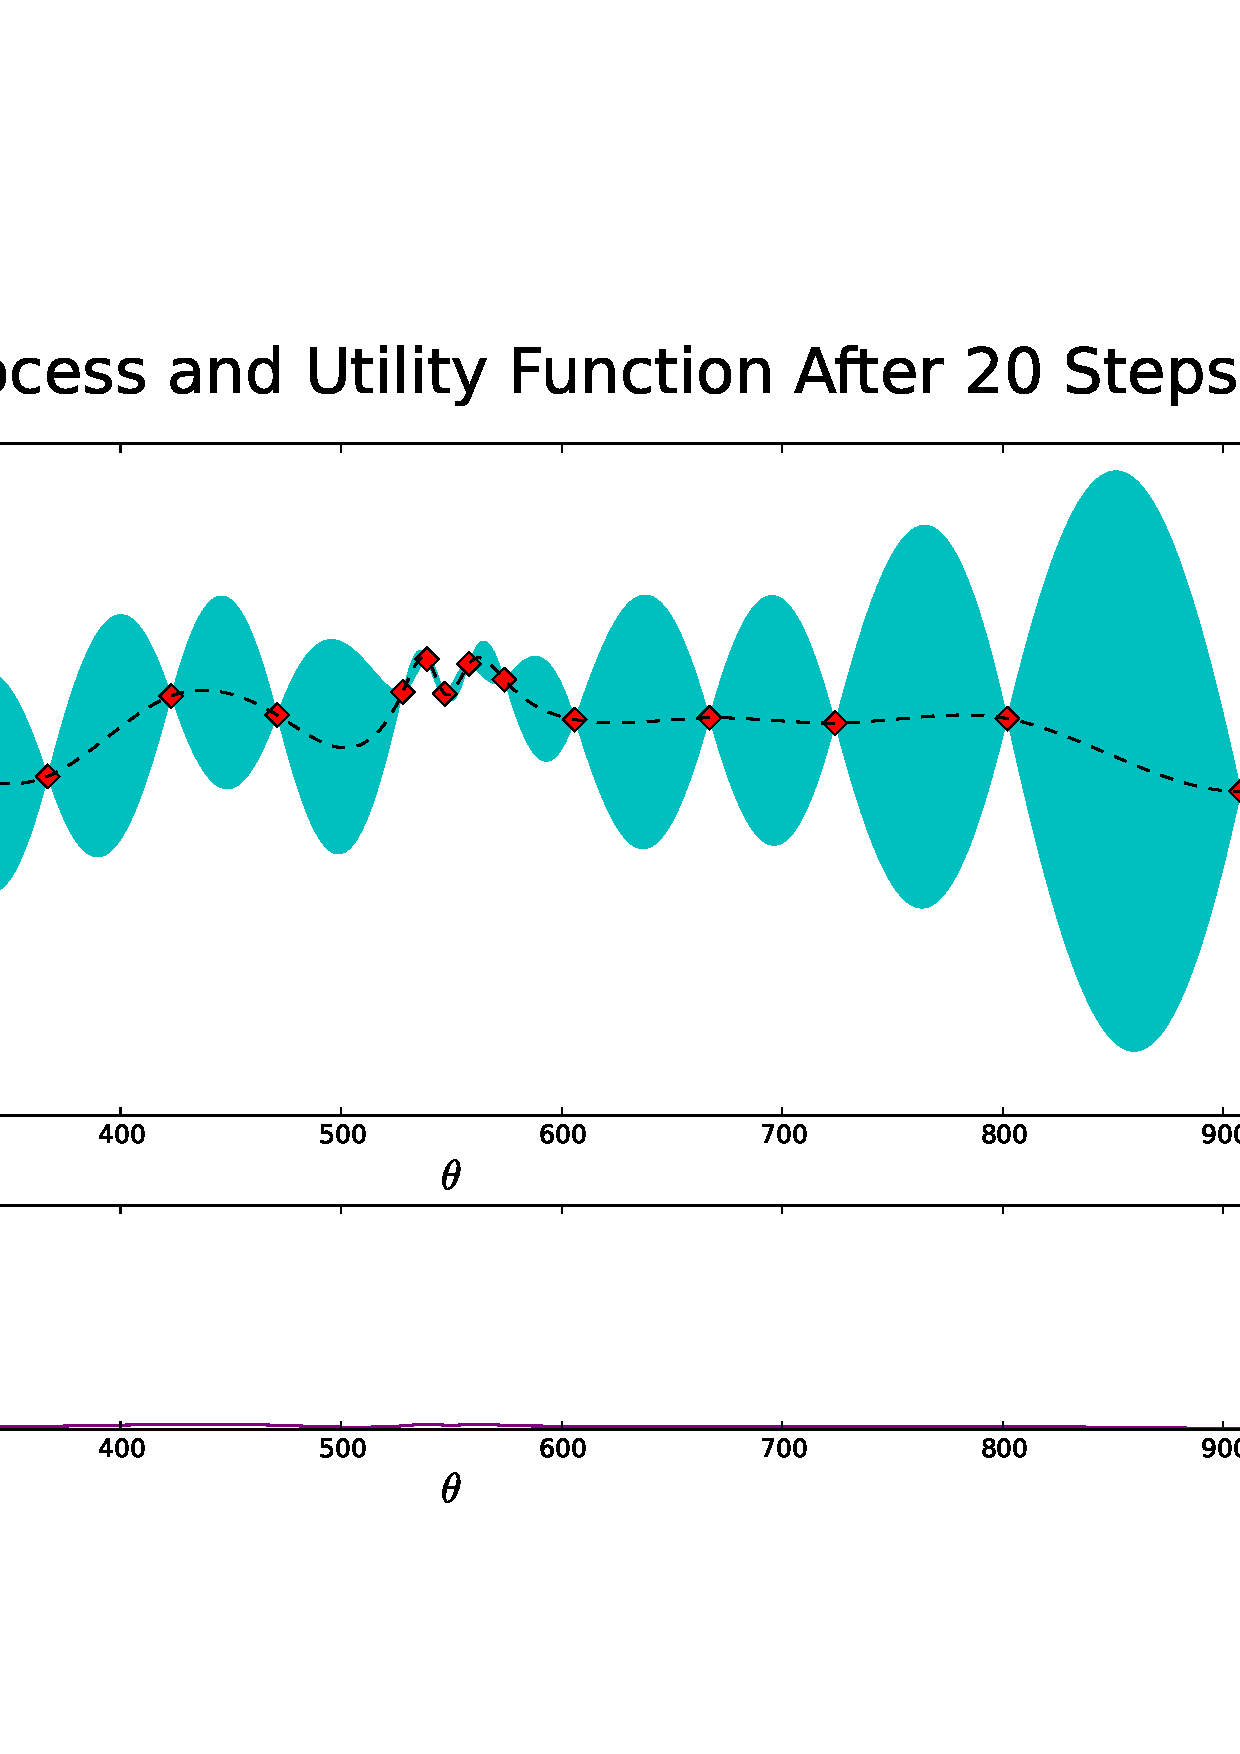
\includegraphics[width=\linewidth]{../../figures/plots/uol_base/plot_b_00__alg_kmeans_pct_100_acq_eips.pdf}
		\end{column}
	\end{columns}
	\begin{center}
		\footnotesize
		Resulting GP approximation with GP-UCB and EIPS acquisition functions used\\
		($k$-Means, \texttt{uol\_bl} environment, 100\% dataset used)
	\end{center}
\end{frame}

\begin{frame}
	\frametitle{Experimental Results}
	\framesubtitle{Multi-Phase Framework - Small Environment}
	\vspace{10pt}
	\begin{columns}
		\begin{column}{0.5\textwidth}
			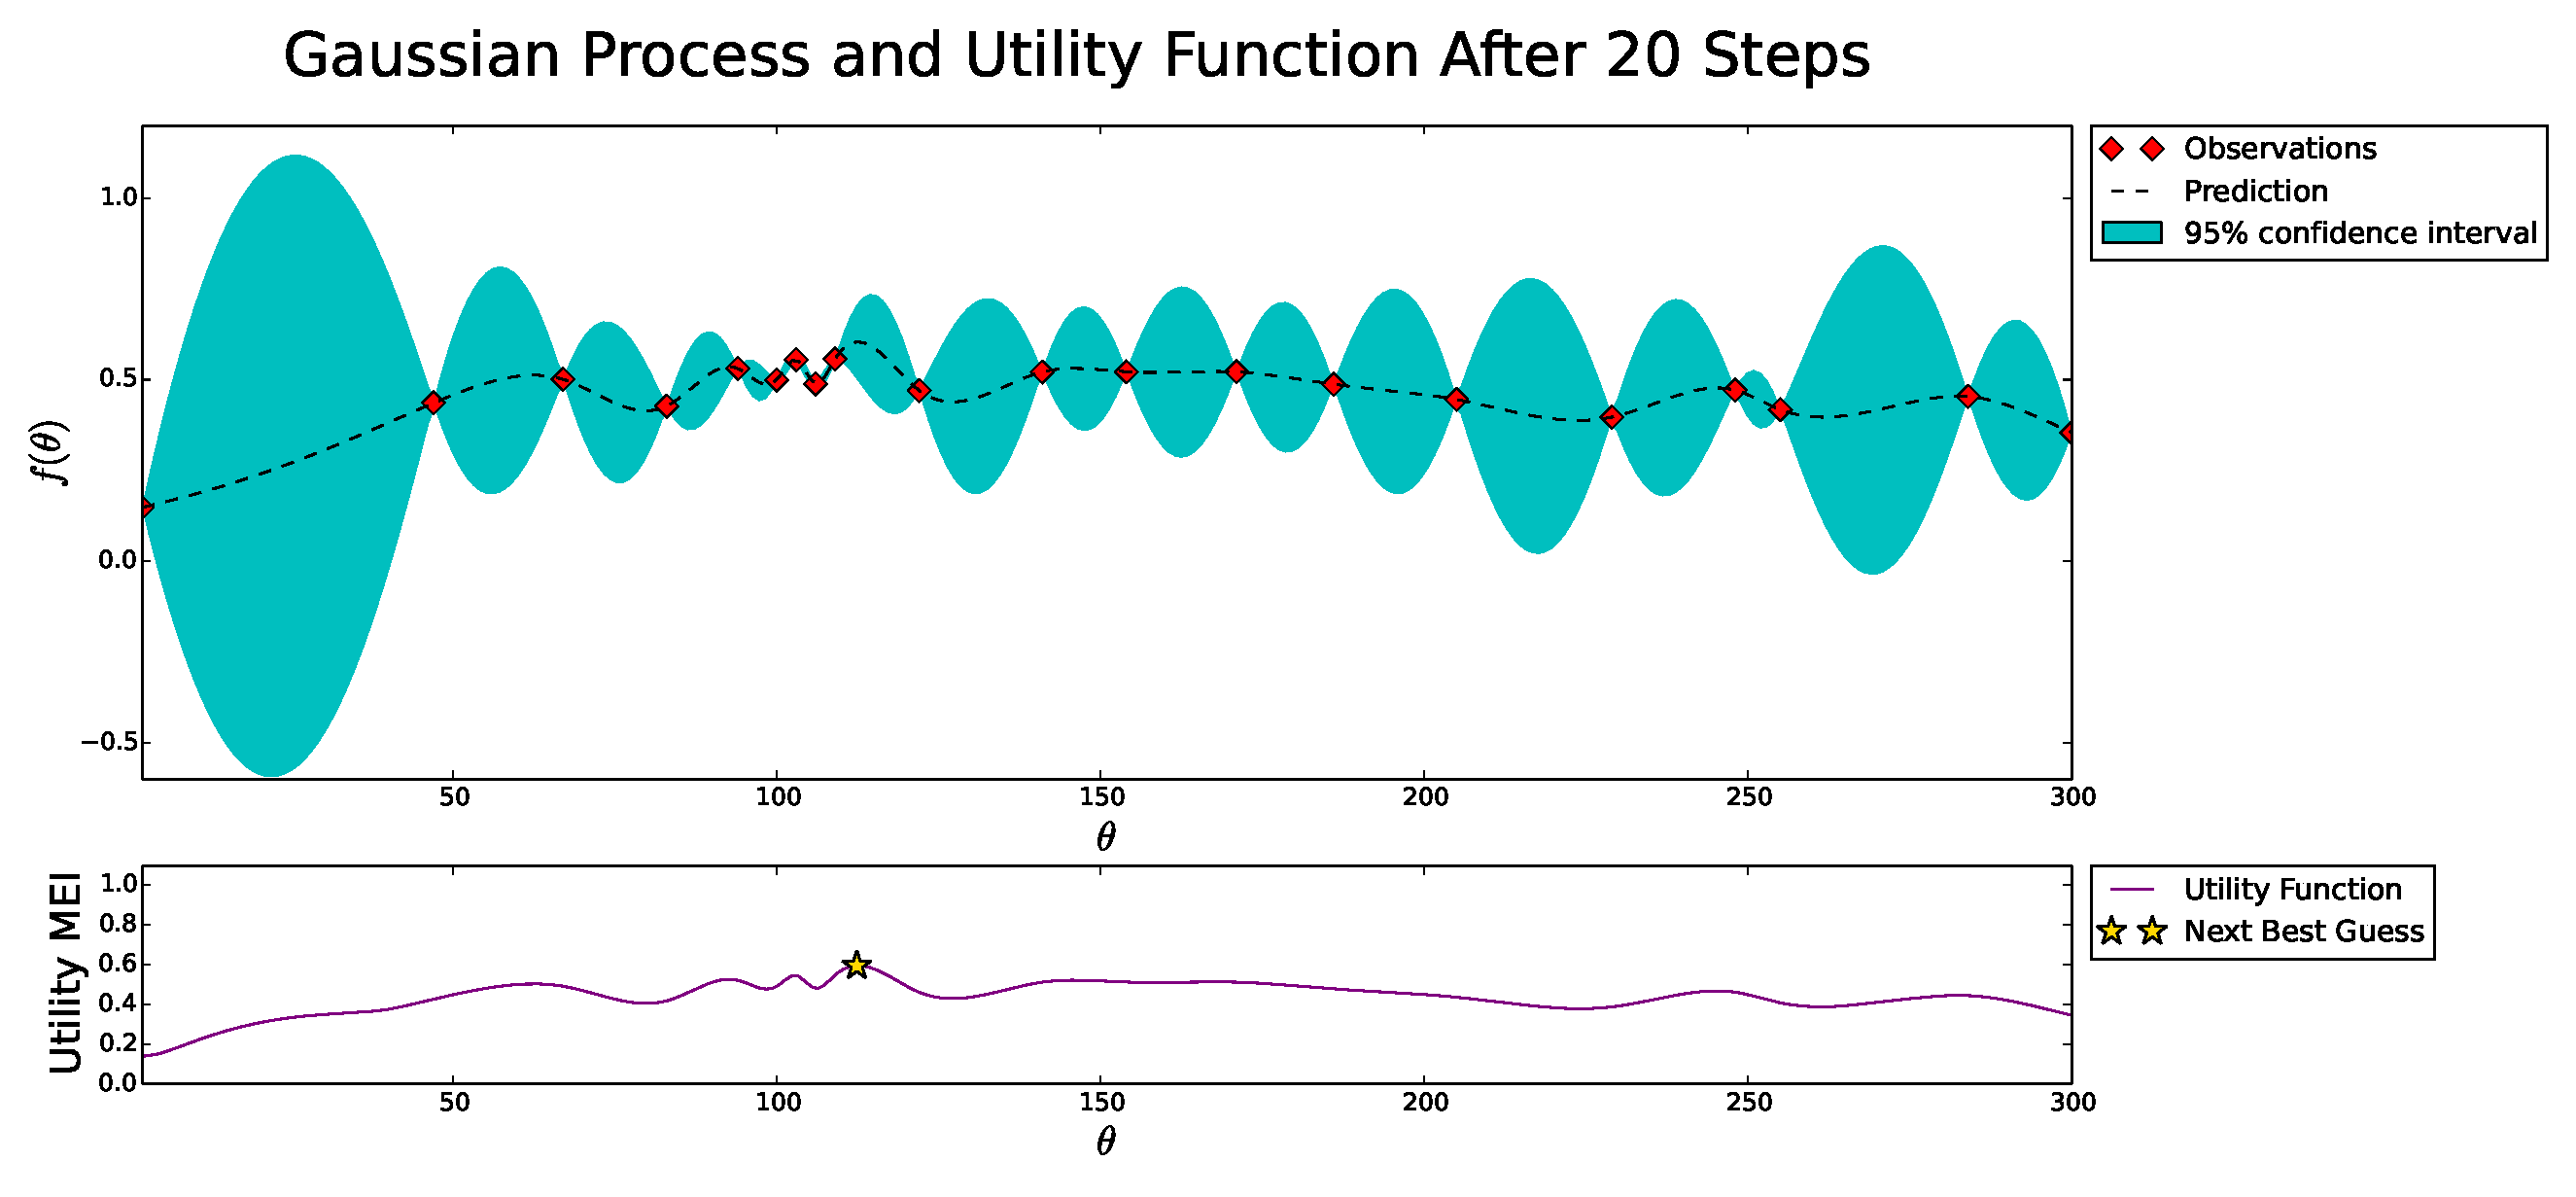
\includegraphics[width=\linewidth]{../../figures/plots/tum_multi/plot_b_00__alg_kmeans_pct_100_acq_ei}
		\end{column}
		\begin{column}{0.5\textwidth}
			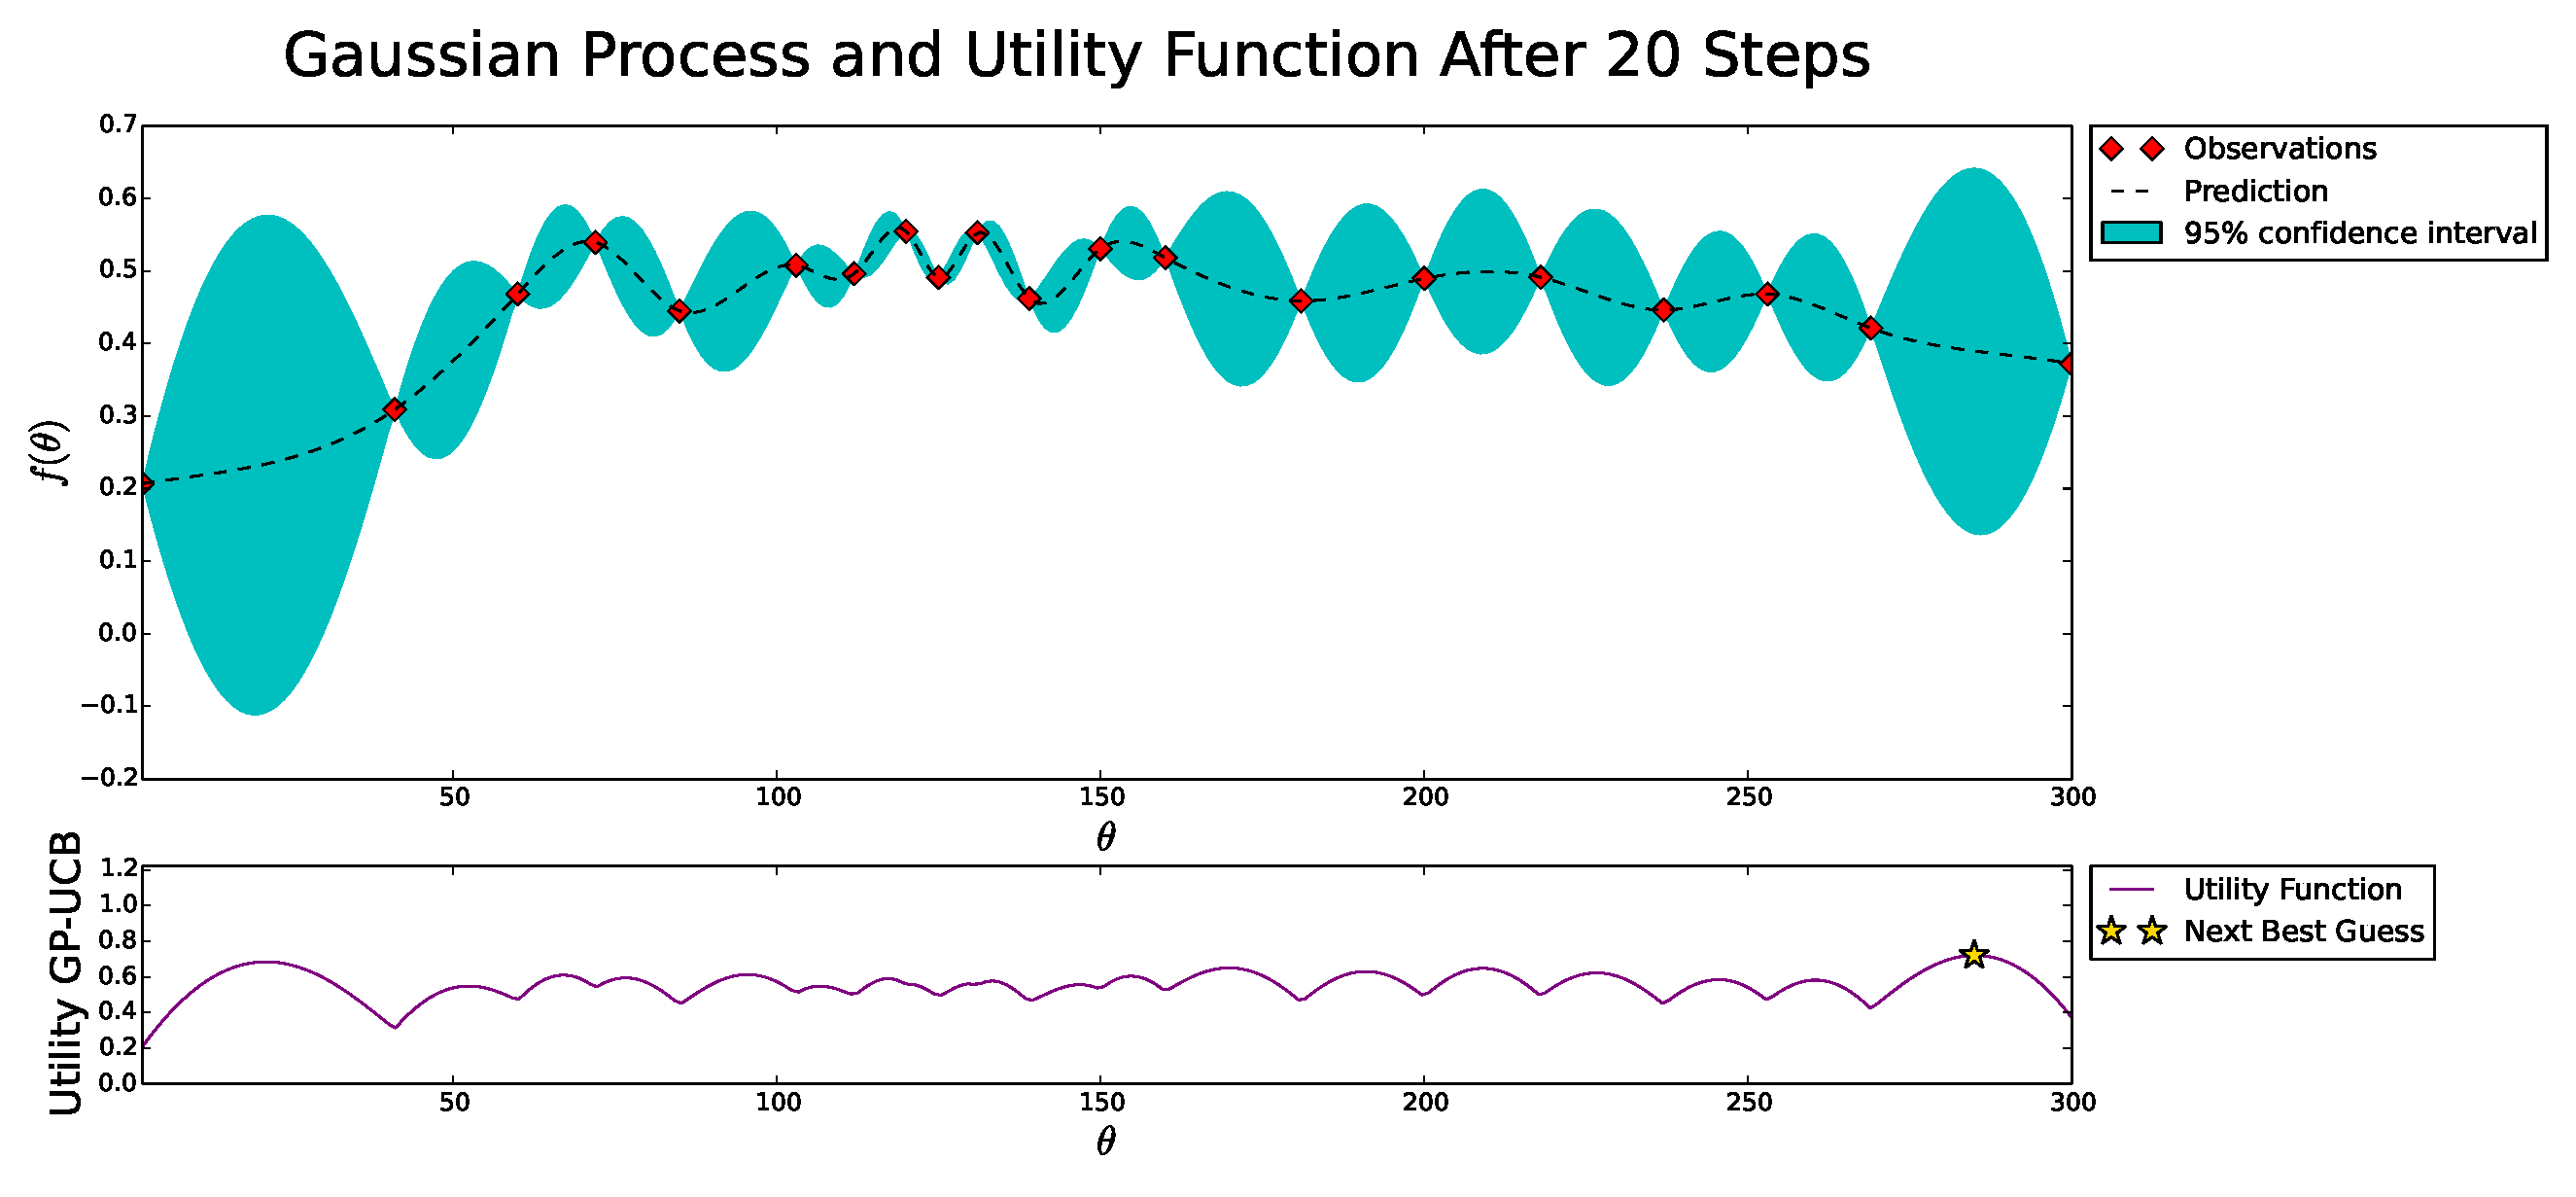
\includegraphics[width=\linewidth]{../../figures/plots/tum_multi/plot_b_00__alg_kmeans_pct_100_acq_ucb}
		\end{column}
	\end{columns}
	\begin{center}
		\footnotesize
		Resulting GP approximation with EI and GP-UCB acquisition functions used in Phase 1\\
		($k$-Means, \texttt{tum\_kitchen} environment, 20 iterations, 100\% dataset used)
	\end{center}
\end{frame}

\begin{frame}
	\frametitle{Experimental Results}
	\framesubtitle{Multi-Phase Framework - Large Environment}
	\vspace{10pt}
	\begin{columns}
		\begin{column}{0.5\textwidth}
			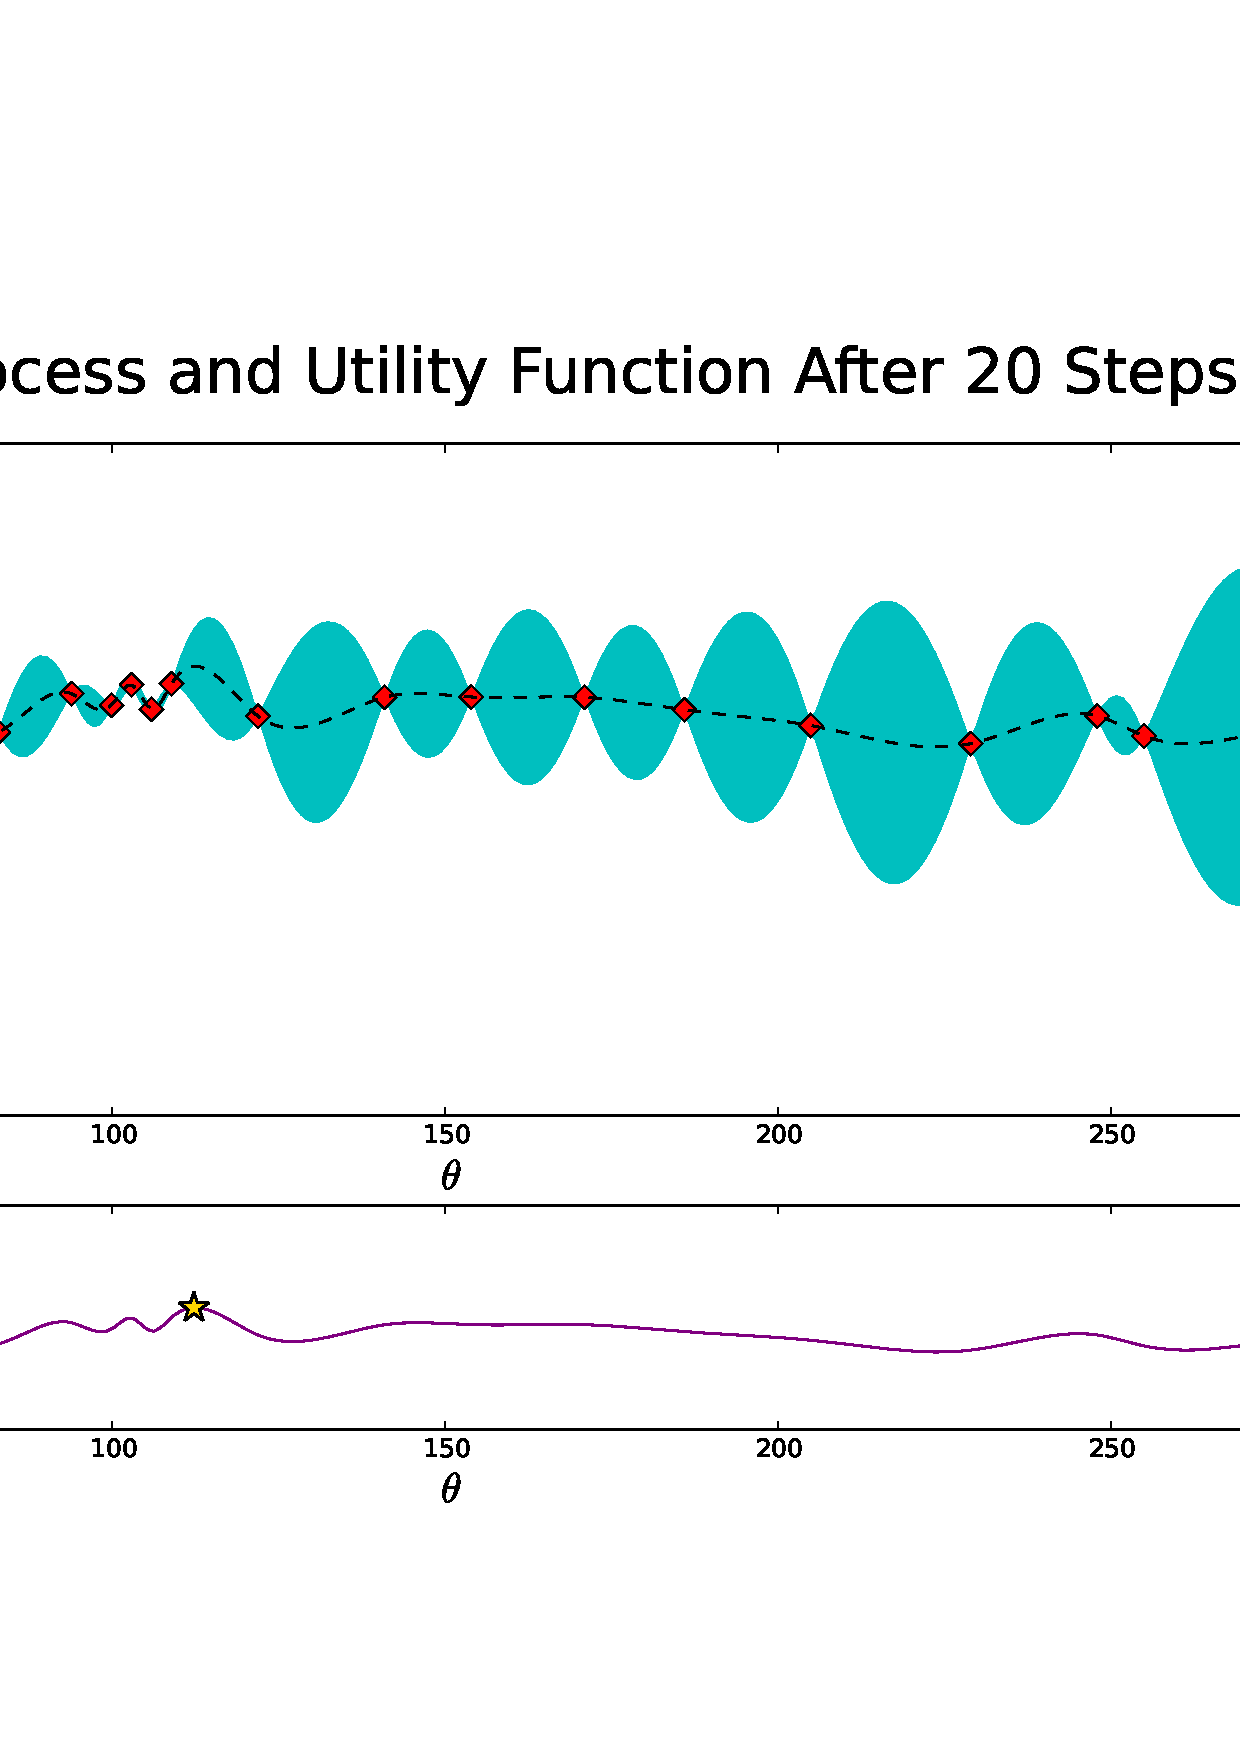
\includegraphics[width=\linewidth]{../../figures/plots/uol_multi/plot_b_00__alg_kmeans_pct_100_acq_ei.pdf}
		\end{column}
		\begin{column}{0.5\textwidth}
			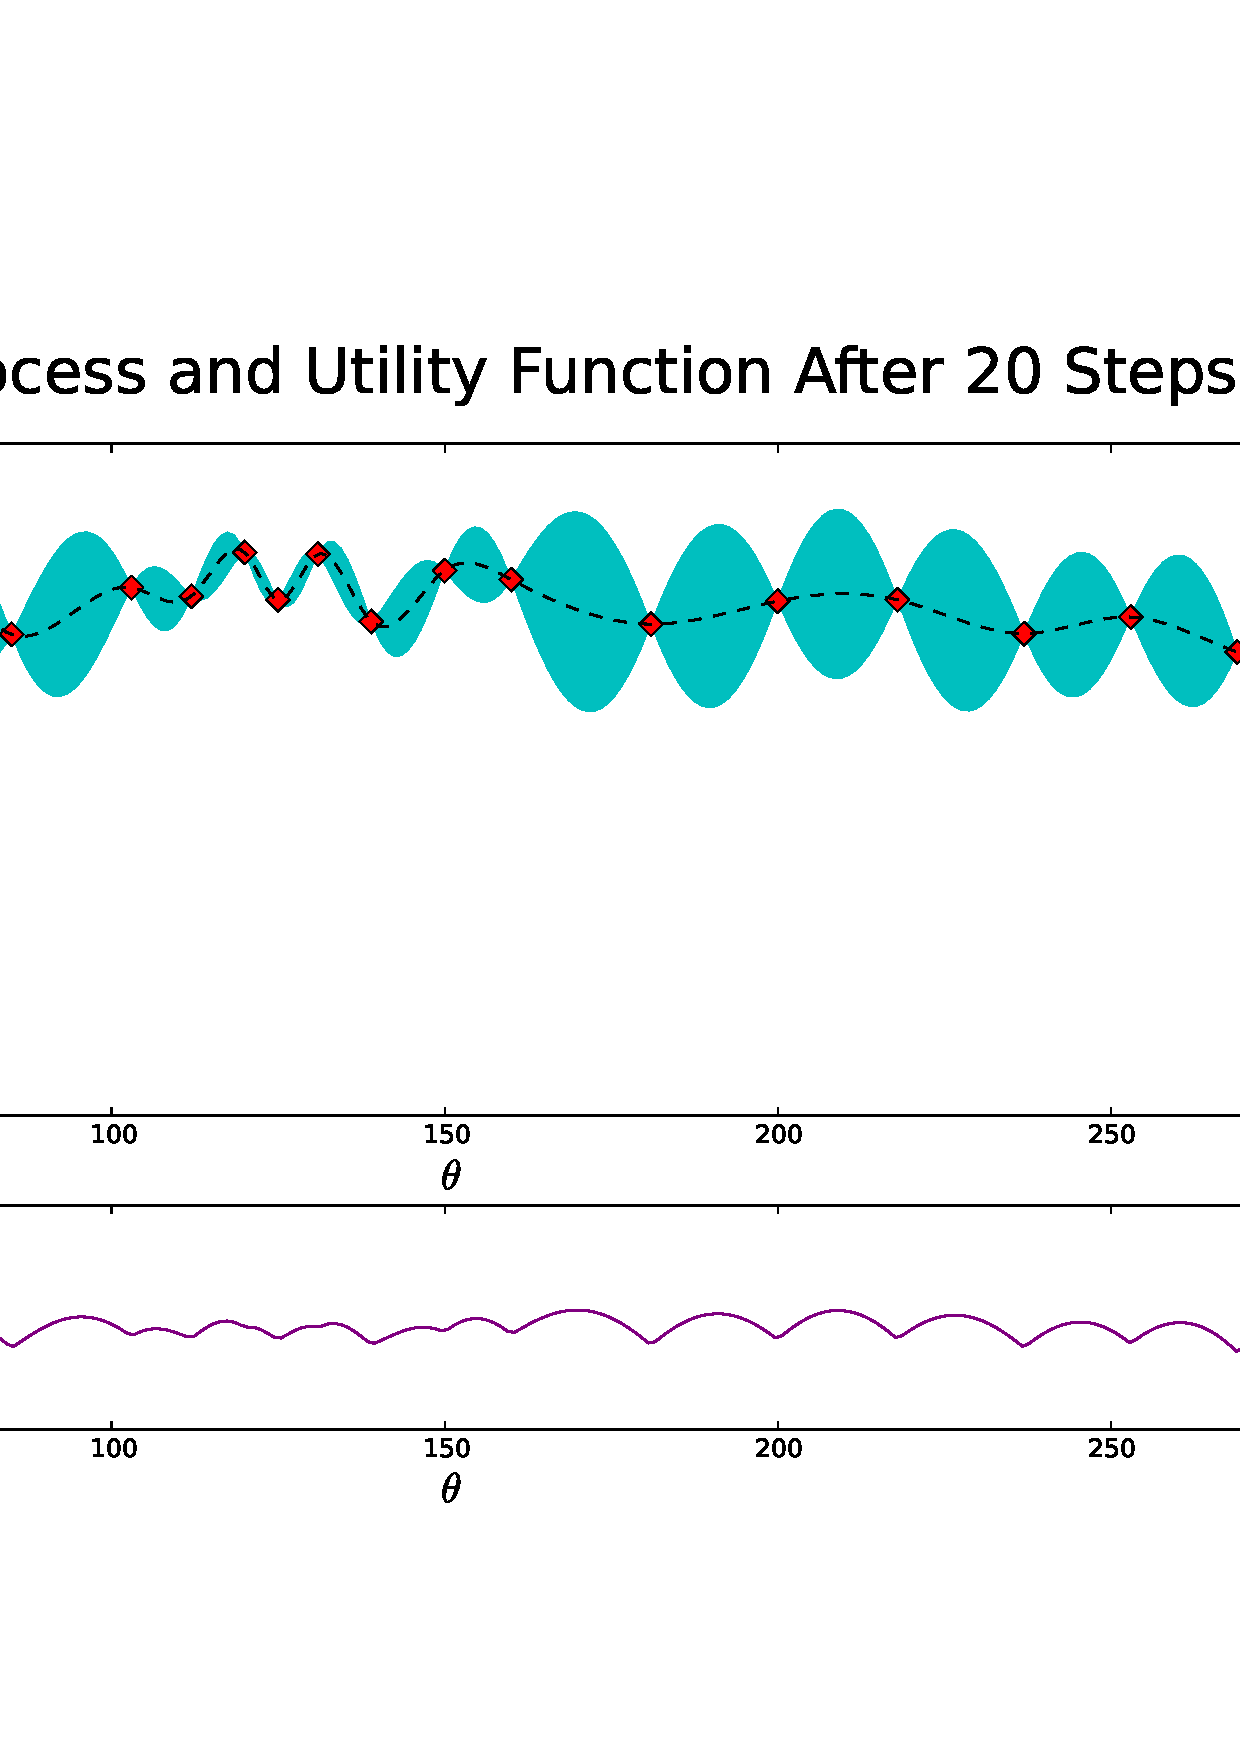
\includegraphics[width=\linewidth]{../../figures/plots/uol_multi/plot_b_00__alg_kmeans_pct_100_acq_ucb.pdf}
		\end{column}
	\end{columns}
	\begin{center}
		\footnotesize
		Resulting GP approximation with GP-UCB and EIPS acquisition functions used\\
		($k$-Means, \texttt{uol\_bl} environment, 30 iterations, 100\% dataset used)
	\end{center}
\end{frame}